\documentclass{article}
\usepackage{graphicx} % Required for inserting images
\usepackage[left=3cm, right=3cm, bottom=3cm, top=3cm]{geometry}	
\usepackage{setspace}
\onehalfspacing
\usepackage{float}
\usepackage{amsmath}
\usepackage{titling} % Allows custom title configuration

\title{Markowitz Portfolio Optimization with Inflation}
\author{Pablo Duce Cabeza \\ Sergey Mirzoev \\ Marc Tschudi}
\date{December 2023}

% Custom title page
\makeatletter
\renewcommand{\maketitle}{
    \begin{titlepage}
        \vspace*{\stretch{1}}
        \begin{center}
            \Large\textbf{\@title}
        \end{center}
        \vspace{\stretch{2}}
        \begin{center}
            \large\@author
        \end{center}
        \vspace{\stretch{3}}
        \begin{center}
            \large\@date
        \end{center}
        \vspace{\stretch{0.5}}
        \begin{center}
            
\includegraphics[width=0.4\textwidth]{figure/uzh_logo_e_pos.eps}
        \end{center}
    \end{titlepage}
}
\makeatother

\begin{document}

\maketitle

\newpage
\tableofcontents
\newpage
\listoffigures
\listoftables
\newpage

\section{Introduction}

The importance of constructing resilient investment portfolios cannot be underestimated in an era marked by economic uncertainties and dynamic financial landscapes. Investors face a constant challenge in preserving and enhancing the real value of their wealth, especially when confronted with the persistent threat of inflation. As inflation erodes purchasing power, traditional investment strategies may prove insufficient, necessitating a paradigm shift towards a more sophisticated approach.

This paper delves into the realm of portfolio optimisation using the renowned Markowitz framework, explicitly focusing on navigating the complexities of an inflationary environment. Rather than adhering to conventional wisdom, our methodology begins with a comprehensive analysis of various asset classes to discern their correlation with inflation. Recognising that not all assets respond uniformly to inflationary pressures, we aim to identify and select those that weather the storm and offer a shield against rising prices' corrosive effects.

The initial phase of our investigation involves an examination of different asset classes, ranging from equities and fixed-income securities to commodities and tangible assets. We seek to unveil the intricate relationships between these asset classes and inflation by scrutinising historical data and employing statistical techniques. Our objective is to discern patterns and identify the investment instruments that exhibit a robust correlation with inflationary trends.

Building on this foundation, we apply the Markowitz portfolio optimisation model. Recognising that optimal portfolios are not one-size-fits-all, we tailor our approach to fixed-income unique characteristics of inflation-sensitive assets. Through a judicious combination of these assets, we aim to construct portfolios that maximise returns and, crucially, hedge against the eroding effects of inflation.

As a result of Markowitz's portfolio optimisation under the spectre of inflation, we show that a portfolio that lies on the efficient frontier compared to an equally weighted portfolio can be constructed. The optimised portfolio substantially outperforms the CPI-adjusted, equally weighted portfolio by strategically selecting assets that exhibit resilience in the face of inflation.

\newpage

\section{Approach}

For an asset class to offer protection against inflation, the asset returns have to be positively correlated with the CPI (Consumer Price Index) when we assume that only long positions can be held; so, when the CPI increases, the asset returns should also increase. The approach we present will be based on filtering. Starting from a large pool of potential assets that could hedge against inflation, we want to understand what are the assets that are more prone to have a positive relationship with inflation. That means analysing the yearly inflation rates and seeing the subsequent returns of a given class. We expect that besides a high correlation with inflation when inflation is very high, returns should also be very high (tail inflation corresponds with the tail of returns). We test the following asset classes and sectors for a hedge against inflation:

\begin{itemize}
    \item XHB: Median Sale Price of Houses Sold in the United States
    \item CPIAUCSL: Consumer Price Index for All Urban Consumers
    \item DCOILWTICO: Crude Oil Prices: West Texas Intermediate (WTI)
    \item GSPC: S\&P 500 Index
    \item GC=F: Gold Futures
    \item GS10: 10-Year Treasury Constant Maturity Rate
    \item GS30: 30-Year Treasury Constant Maturity Rate
    \item VNQ: REITs (Vanguard Real Estate ETF)
    \item DBC: Commodities (Invesco DB Commodity Index Tracking Fund)
    \item FXE: Foreign Currencies (Currency Shares Euro Trust)
    \item BTC-USD: Cryptocurrencies (Bitcoin)
    \item IGF: Infrastructure Funds (iShares Global Infrastructure ETF)
    \item XLE: Energy Stocks (Energy Select Sector SPDR Fund)
\end{itemize}

\subsection{Visual inspection}

Visual inspection is a rapid way to determine if there's a relationship between the different asset classes. We look at the time series of the Log Returns of both the adjusted and non-adjusted returns to see potential relationships. Although this is unclear, it allows us to draw the first conclusions. In figure \ref{fig:mesh2} on page \pageref{fig:mesh2}, we can see that bonds (GS10, GS30) are very very closely related and also follow CPI. We also can see a relationship between DBC (commodities) and XLE (energy).

\begin{figure}
    \centering
    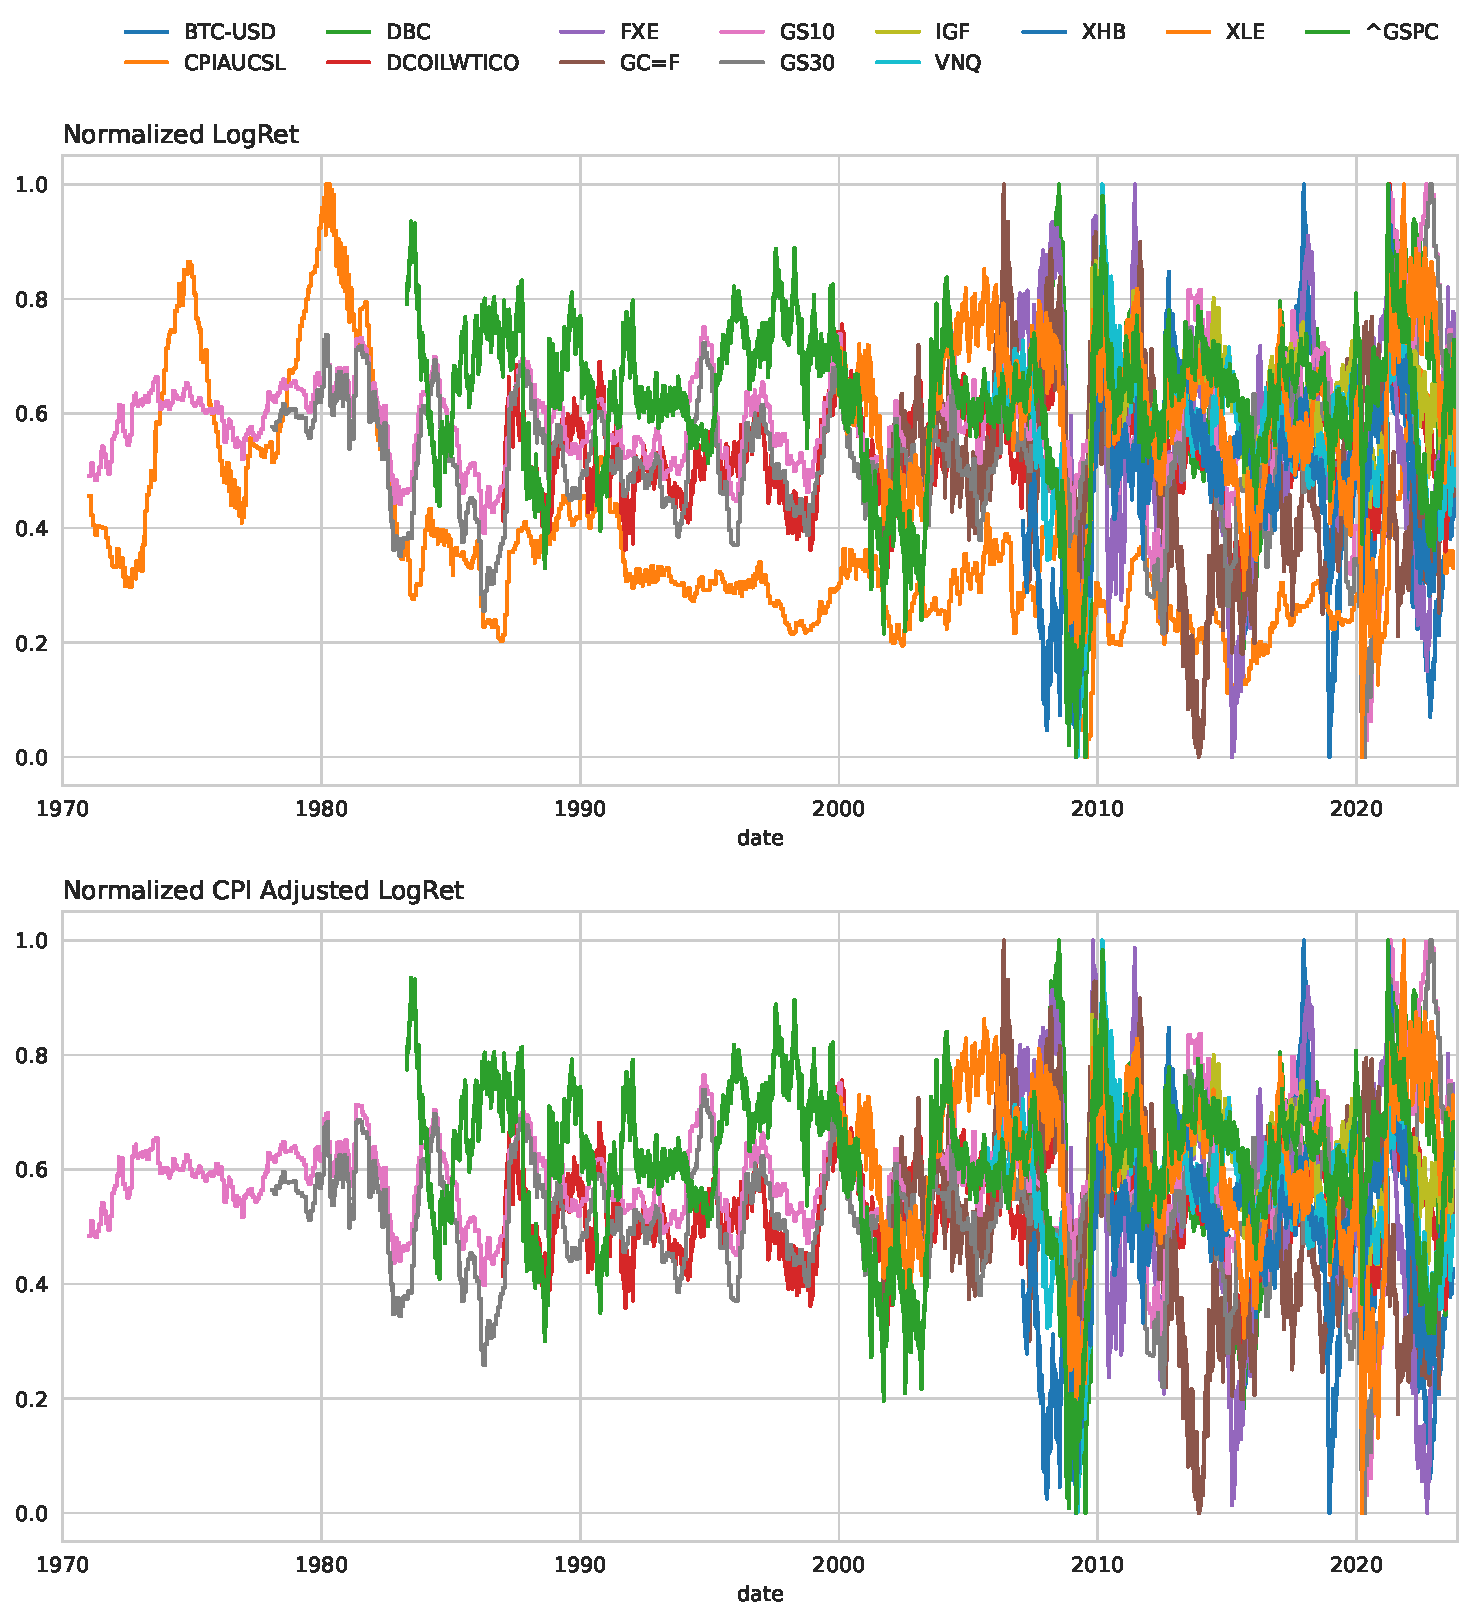
\includegraphics[width=1\textwidth]{figure/Normalized_Returns.pdf}
    \caption{Normalised Yearly Rolling Log-Returns of different Asset Classes.}
    \label{fig:mesh2}
\end{figure}

\subsection{Facet Grid}

We plotted a Facet Grid of the returns and CPI to see further the first visual relation between the asset classes and CPI (figure \ref{fig:mesh6}). Especially the commodities and the energy sectors show a robust positive relationship according to these plots. The gold futures (GC=F) and foreign currencies (FXE) plots are interesting to see. The relationship is generally strongly positive up to point 0.4 in the CPI data. Some data points between 0.4 and 0.6 lie, which pulls the linear relationship downwards. Because it's a linear plot, the fewer points after 0.4 than before 0.4 skew the relation downwards; if one corrects for this, the relationship between the asset class and CPI would be strongly positive.

\begin{figure}[H]
    \centering
    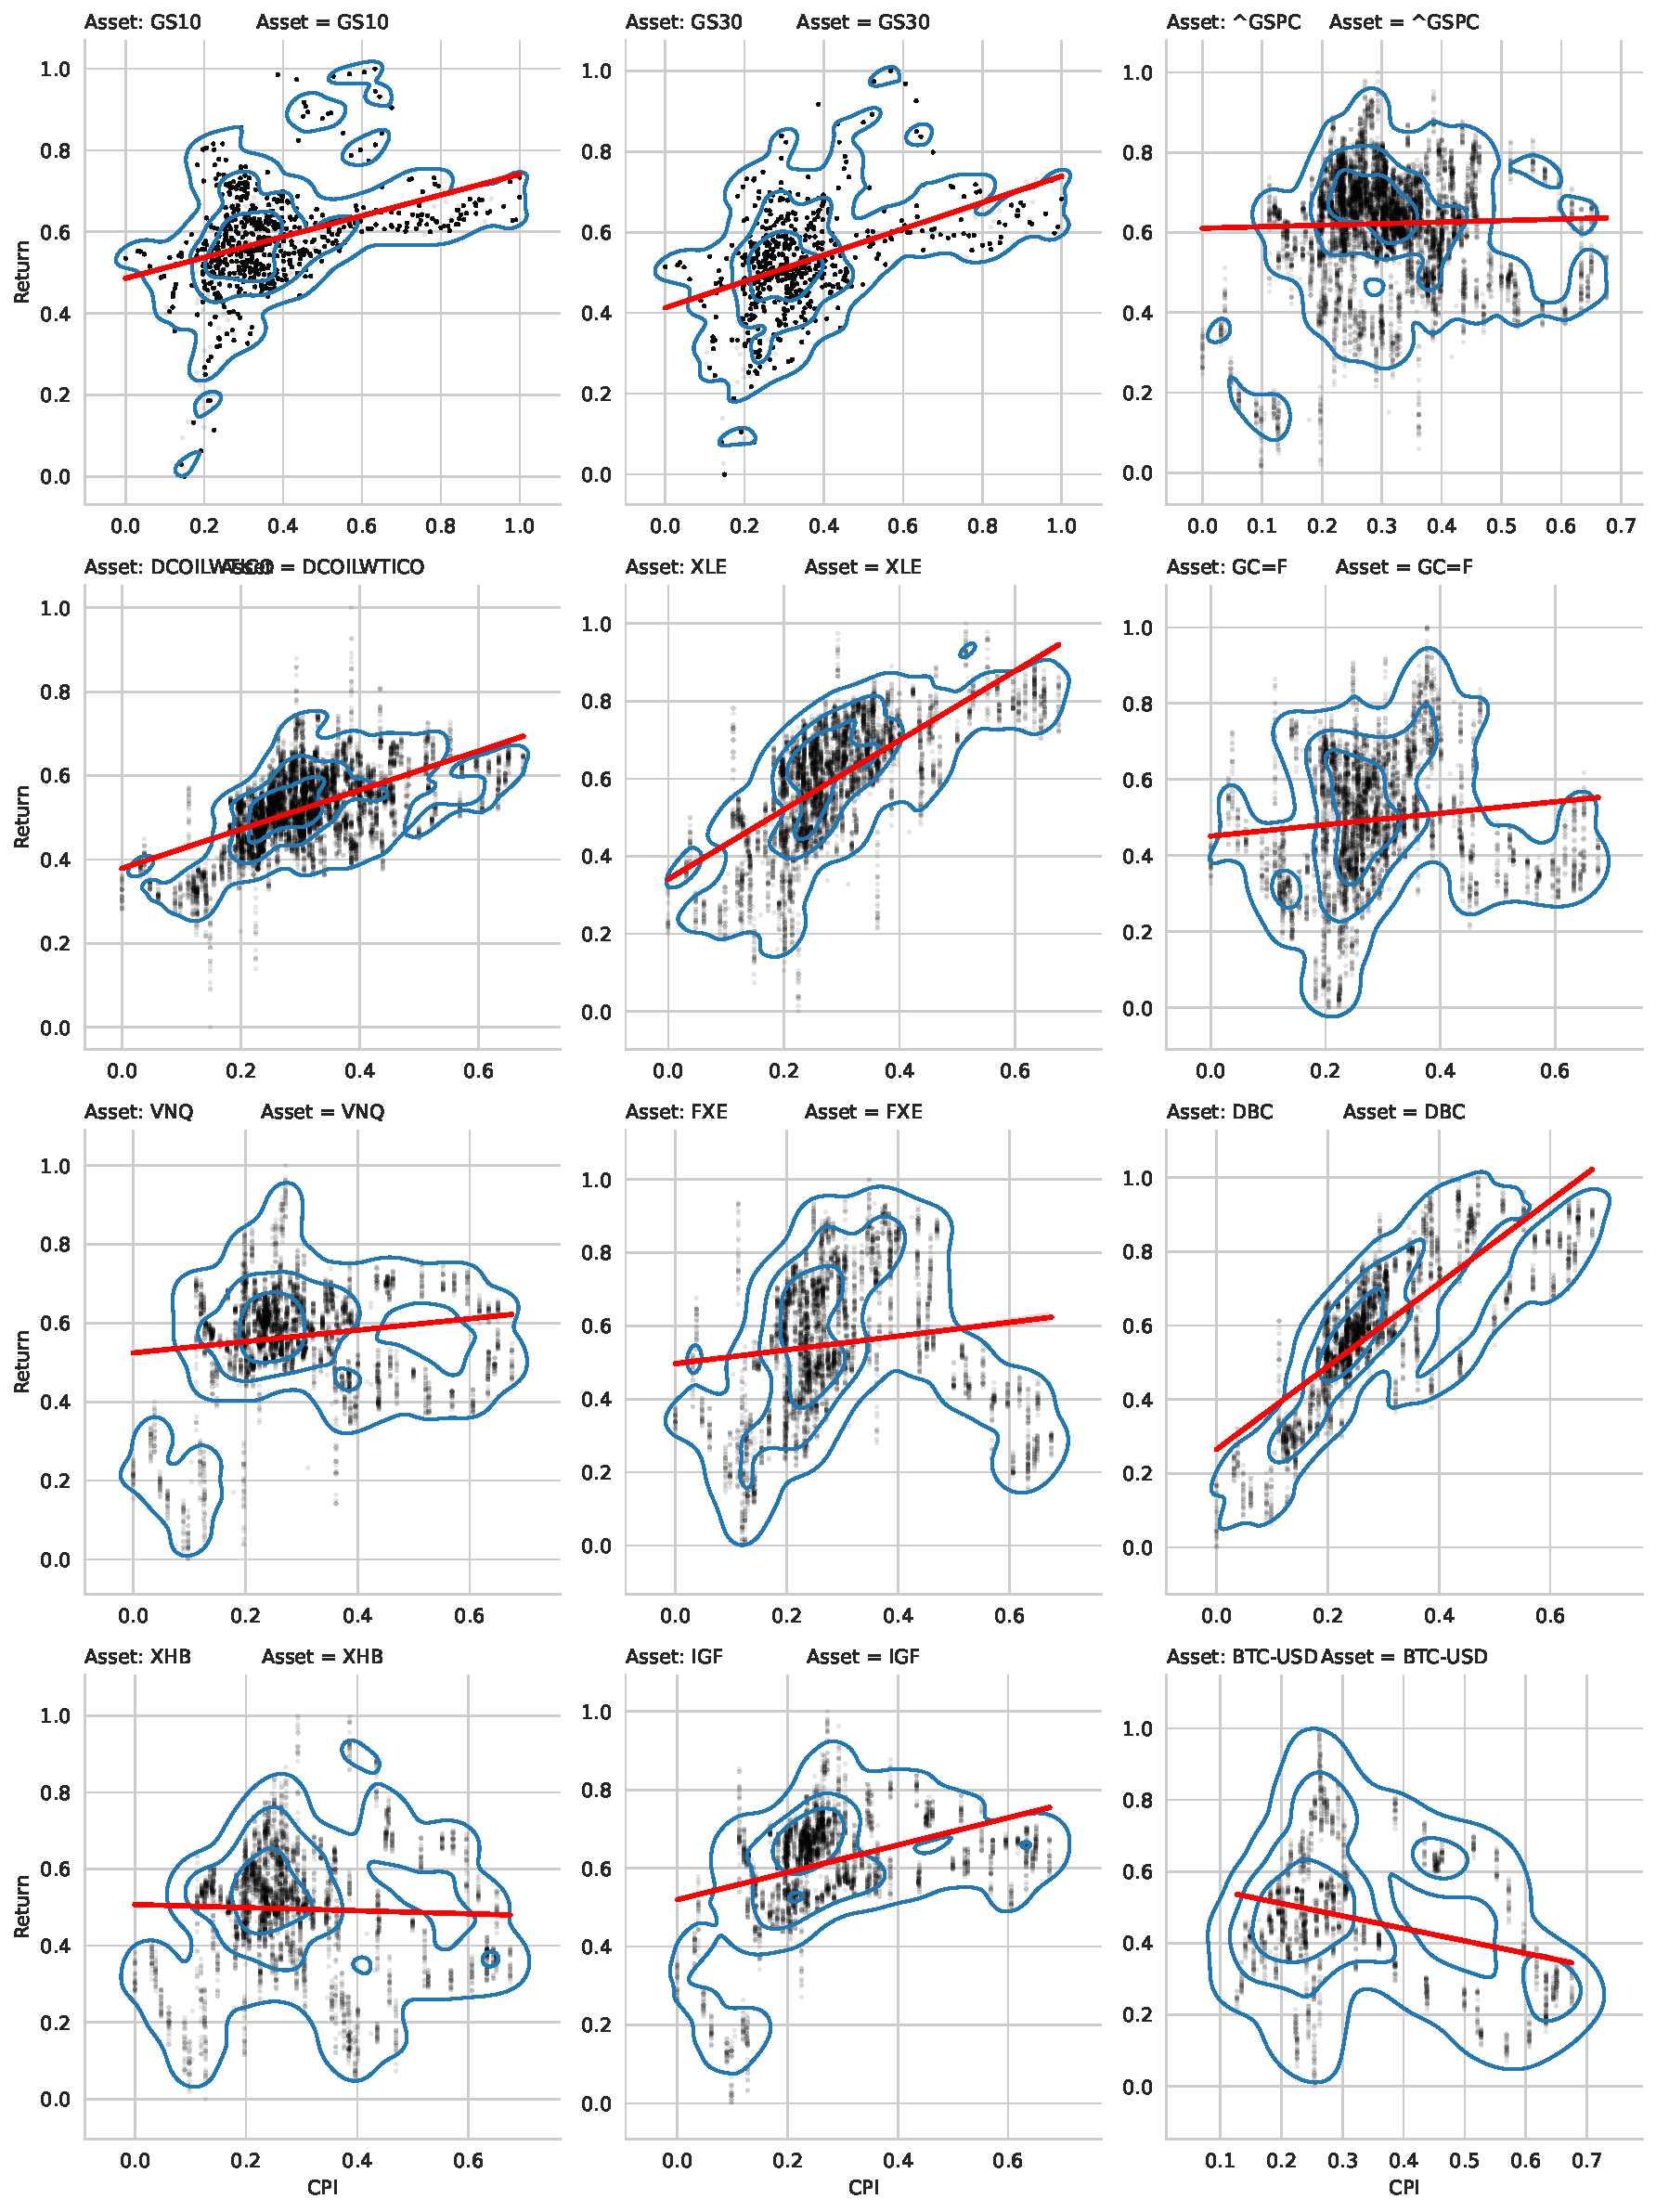
\includegraphics[width=1\textwidth]{paper/figure/CPI_Returns.pdf}
    \caption{Facet Grid of each Asset Class against the CPI.}
    \label{fig:mesh6}
\end{figure}

\subsection{Correlation}

A high correlation shows a linear relationship between the data. Using our data of yearly returns (rolling 1Y log returns), we can compute the pairwise correlation (correlation matrix). We are interested in the correlation between the CPI (CPIAUSCL) and a given asset class. The reason to compute the correlation in the returns and not in the prices is that we can assume that returns are independent and identically distributed. Based on this result, we can observe that Energy ETF (XLE), Bonds (GS10, GS30), Oil (DCOILWTICO), and Commodities (DBC)... are significantly positively correlated with inflation.

\begin{figure}[H]
    \centering
    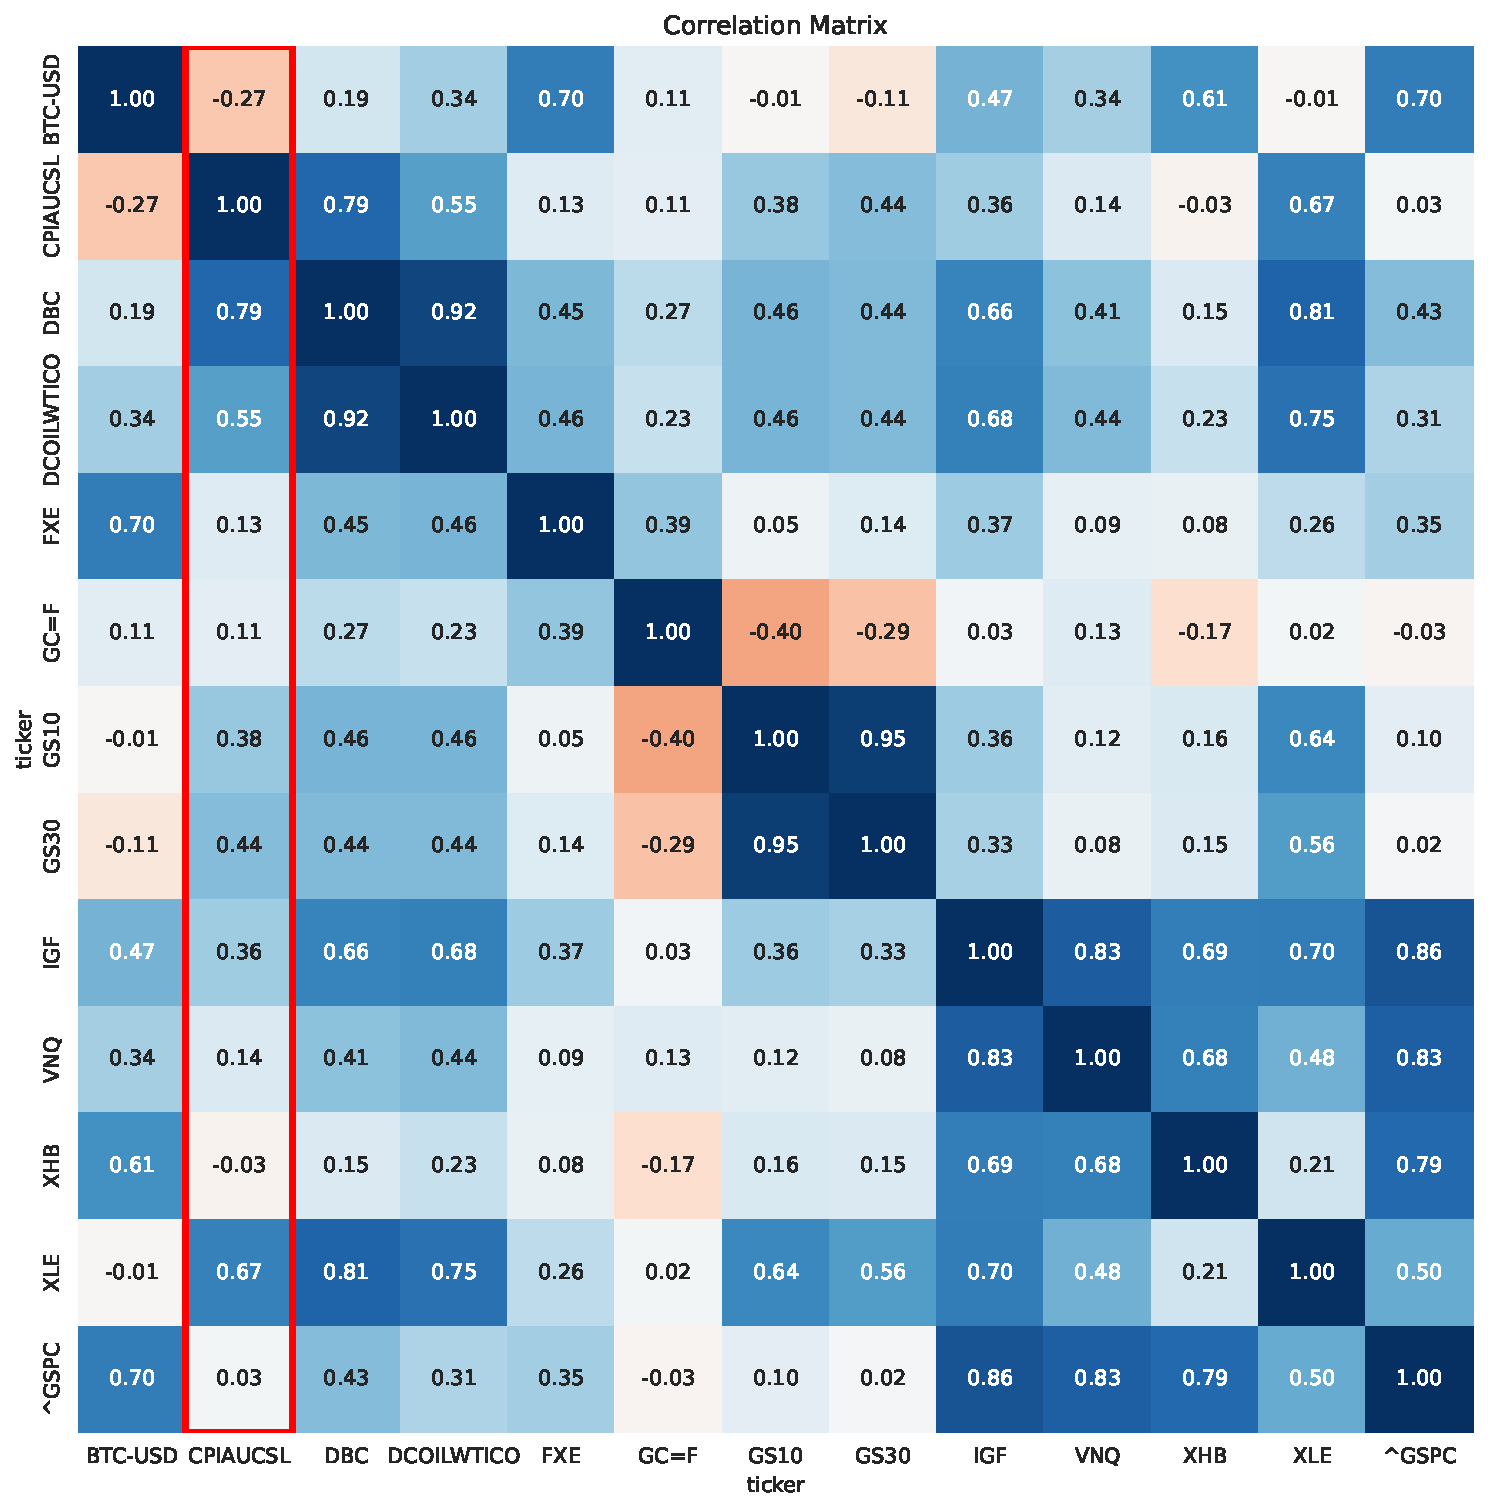
\includegraphics[width=0.8\textwidth]{figure/Correlation_Matrix.pdf}
    \caption{Correlation Matrix.}
    \label{fig:mesh1}
\end{figure}

\subsection{Cointegration}

Based on the understanding of correlation in financial data, we can extend our analysis to explore the concept of cointegration. Cointegration is a statistical property of a collection of time series variables, indicating a long-term equilibrium relationship between them. Unlike correlation, which merely identifies the linear relationship in the level of data, cointegration delves deeper by detecting a link in their long-term trends despite short-term deviations.

In our case, examining cointegration among assets like the Energy ETF (XLE), Bonds (GS10, GS30), Oil (DCOILWTICO), Commodities (DBC), and inflation metrics such as the CPI, would be insightful. This is particularly important because financial markets often exhibit trends and mean-reverting behaviour over extended periods. While correlation informs us about the degree of linear relationship in the returns, cointegration helps us understand the extent to which these asset classes move together over time, bound by an equilibrium relationship.

By investigating cointegration, we can assess whether any discrepancies between these assets and inflation are temporary or indicative of a fundamental shift. This understanding is crucial for long-term investment strategies and risk management, as it helps identify pairs or groups of assets that are likely to move in sync over time. Such analysis is especially relevant in market conditions characterised by significant economic changes, where long-term relationships might be more stable and reliable than short-term correlations.

\begin{figure}[H]
    \centering
    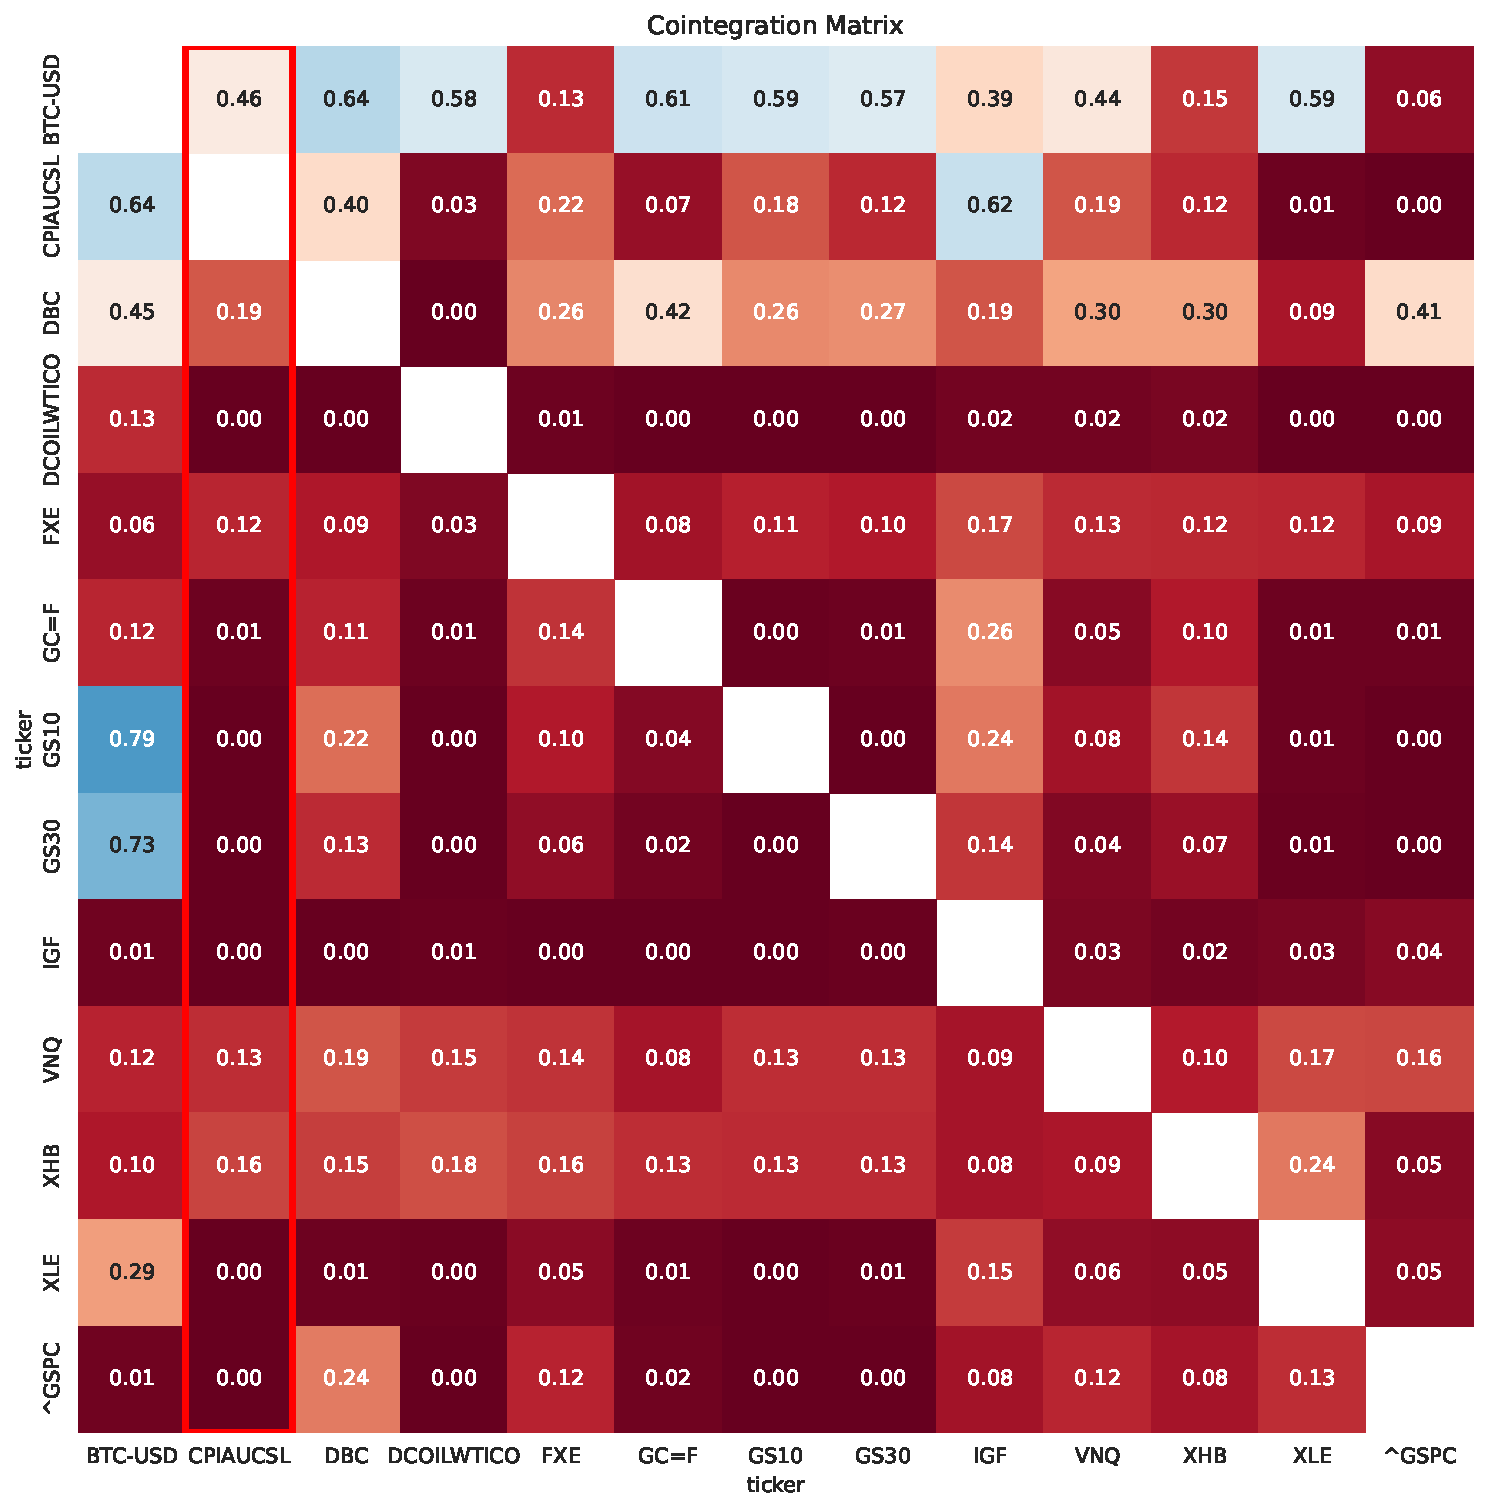
\includegraphics[width=0.8\textwidth]{paper/figure/Cointegration_Matrix.pdf}
    \caption{Cointegration Matrix.}
    \label{fig:mesh3}
\end{figure}

\section{Results}

In the following part, we describe our approach and the results in more detail. 

\subsection{The Concept of Portfolio Optimization}

\subsubsection*{Efficient Frontier}

The heart of Markowitz's theory is the "Efficient Frontier," a graphical representation showing the optimal set of portfolios providing the maximum possible expected return for a given level of risk. Portfolios that lie below the efficient frontier are sub-optimal because they do not provide enough return for the level of risk they carry.

\subsubsection*{Risk and Return}

In Markowitz's framework, risk is quantified as the standard deviation of portfolio returns, a measure of variability in returns. Return is the expected return of the portfolio, a weighted sum of the expected returns of the individual assets.

\subsection{Mathematical Formulation}

\subsubsection*{Expected Portfolio Return}

The expected return of a portfolio is the weighted sum of the returns of the individual asset classes:

\begin{equation}
R_p = \sum_{i=1}^{n} w_i \times R_i
\end{equation}

where \( R_p \) is the expected portfolio return, \( n \) is the number of assets in the portfolio, \( w_i \) is the weight of the asset \textit{i}, and \( R_i \) is the expected return of the asset \textit{i}.

\subsubsection*{Portfolio Variance}

The risk of the portfolio is often quantified by its variance and is given by:

\begin{equation}
\sigma_p^2 = \sum_{i=1}^{n} \sum_{j=1}^{n} w_i \times w_j \times \sigma_{ij}
\end{equation}

where \( \sigma_p^2 \) is the portfolio variance, \( \sigma_{ij} \) is the covariance between the returns of assets \textit{i} and \textit{j}.

\subsubsection*{Sharpe Ratio}

The Sharpe ratio is used to measure the risk-adjusted return of the portfolio. It puts the portfolio return into relation with the portfolio's standard deviation and is calculated as follows:

\begin{equation}
\text{Sharpe Ratio} = \frac{R_p - R_f}{\sigma_p}
\end{equation}

where \( R_f \) is the risk-free rate.

Because we already adjusted the returns for the CPI data, the risk-free rate is 0 in this case.

\subsection{The Optimisation Problem}

The portfolio optimisation aims to find the set of weights \( \{ w_i \} \) that maximises the Sharpe ratio or, alternatively, minimises the negative Sharpe ratio.

\subsubsection*{Method}

The optimisation is typically performed using numerical methods, such as the Sequential Least Squares Programming (SLSQP) algorithm used in the provided Python code. This algorithm is commonly used for solving nonlinear constrained optimisation problems. It belongs to the class of sequential quadratic programming methods and is particularly effective for problems with nonlinear objective functions and constraints.

The primary goal of the SLSQP algorithm is to find the values of the decision variables that minimise or maximise a given objective function, subject to a set of constraints. In mathematical terms, the algorithm aims to solve problems of the form:

Minimise or maximise \( f(x) \) subject to:
\begin{itemize}
    \item \( c_j(x) = 0, \quad j = 1, \ldots, m \) (equality constraints)
    \item \( c_k(x) \geq 0, \quad k = 1, \ldots, n \) (inequality constraints)
\end{itemize}

Here, \( x \) represents the vector of decision variables, \( f(x) \) is the objective function, and \( c_j(x) \) and \( c_k(x) \) are the equality and inequality constraints, respectively.
The SLSQP algorithm iteratively refines its solution by approximating the objective function and constraints using quadratic models. It combines aspects of the Sequential Quadratic Programming (SQP) method with least squares minimisation. The algorithm proceeds through a series of iterations, adjusting the decision variables to achieve an optimal solution while satisfying the constraints.

Overall, the Sequential Least Squares Programming algorithm is a versatile optimisation tool suitable for various nonlinear-constrained optimisation problems. It is particularly valuable in multiple fields, including finance, engineering, and scientific research.

\subsection{Optimization Results}

Based on our asset class selection methodology and optimisation, we have the final portfolio, which is listed in Table 1. For the optimisation problem, we put in place the following two constraints to ensure a level of diversification in the final portfolio:

\begin{itemize}
    \item The sum of the weights must equal 1: \( \sum_{i=1}^{n} w_i = 1 \).
    \item Each weight must be within predefined bounds of 5\% and 30\%.
\end{itemize}

With these constraints, we get the following final portfolio:

\begin{table}[H]
\centering
\begin{tabular}{ | c | c | }
 \hline
 \textbf{Asset Class} & \textbf{Weight} \\
 \hline
 GS10: 10-Year Treasury Constant Maturity Rate & 5\% \\ 
 \hline
 GS30: 30-Year Treasury Constant Maturity Rate & 5\% \\
 \hline
 DCOILWTICO: Crude Oil Prices: West Texas Intermediate (WTI) & 5\% \\ 
 \hline
 XLE: Energy Stocks (Energy Select Sector SPDR Fund) & 15\% \\ 
 \hline
 GC=F: Gold Futures & 30\% \\ 
 \hline
 FXE: Foreign Currencies (CurrencyShares Euro Trust) & 5\% \\
 \hline
 DBC: Commodities (Invesco DB Commodity Index Tracking Fund) & 5\% \\ 
 \hline
 BTC-USD: Cryptocurrencies (Bitcoin) & 30\% \\ 
 \hline
\end{tabular}
 \label{table:tab1}
 \caption{Optimised Portfolio Composition.}
\end{table}

In figure \ref{fig:mesh4}, the CPI-adjusted optimised portfolio is compared to the CPI-adjusted equally weighted portfolio as a benchmark. Our optimised portfolio can substantially outperform the portfolio that does not consider inflation in its composition.

Possible random portfolios were simulated in figure \ref{fig:mesh5}. The optimised portfolio marked by a red star lies precisely on the efficient frontier, meaning that no higher return (lower risk) can be achieved with the given risk (return).

In the following table, one can find the presented measures mentioned at the beginning of chapter 3. The volatility is strongly influenced by the overweight of the asset class cryptocurrencies (Bitcoin):

\begin{table}[H]
\centering
\begin{tabular}{ | c | c | }
 \hline
 \textbf{Measure} & \textbf{Result} \\
 \hline
 Expected Annual Return & 9.82\% \\ 
 \hline
 Risk (Annual standard deviation) & 19.96\% \\
 \hline
 Sharpe Ratio 0.4922 & 0.4922 \\ 
 \hline
\end{tabular}
 \label{table:tab2}
 \caption{KPIs.}
\end{table}

\begin{figure}[H]
    \centering
    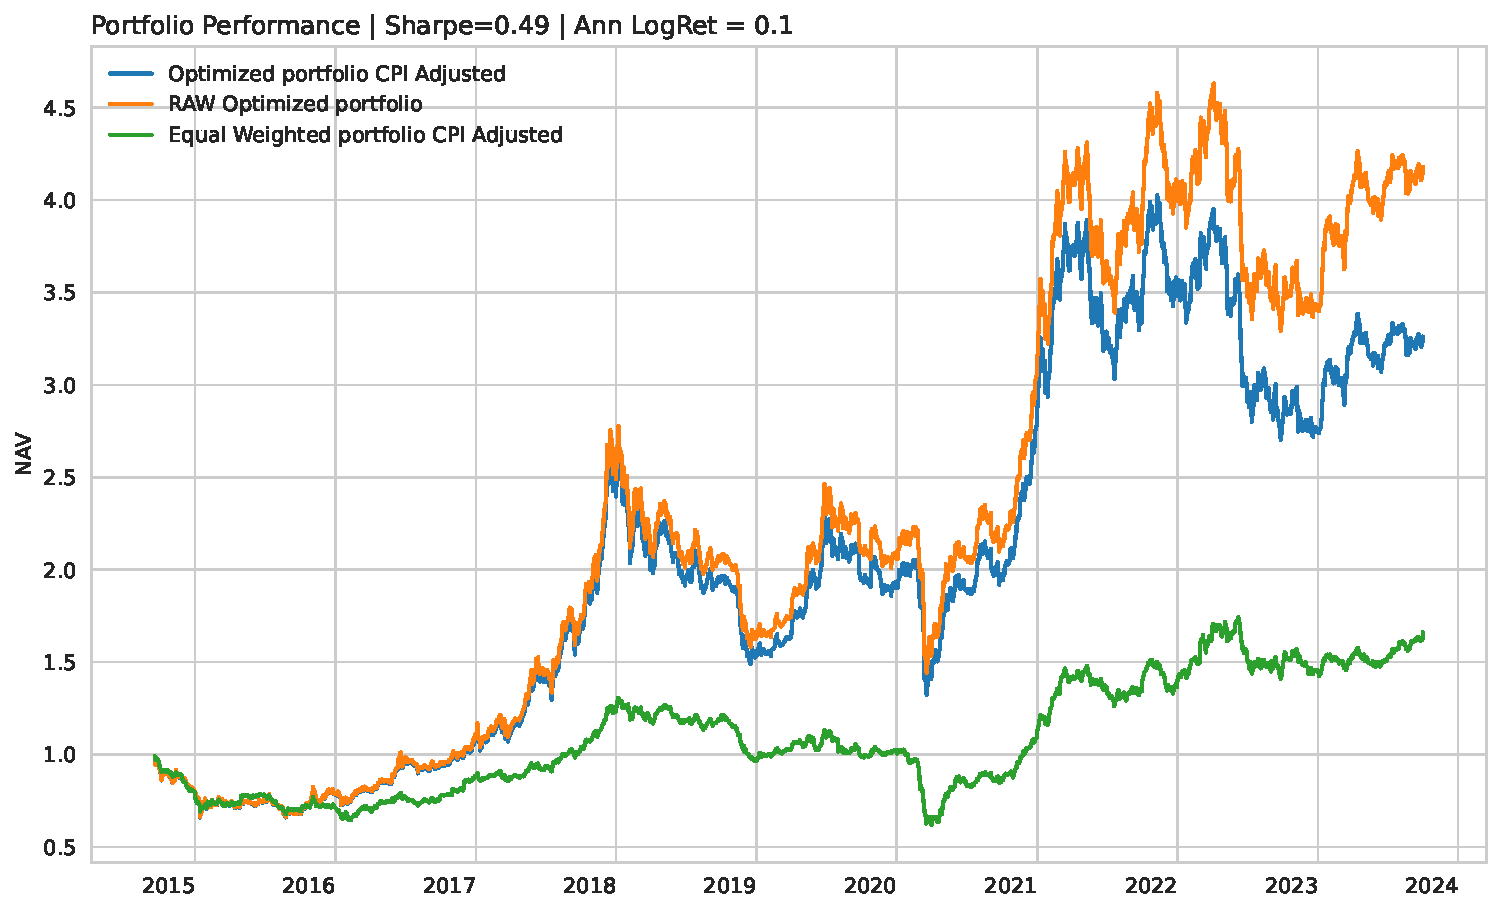
\includegraphics[width=1\textwidth]{paper/figure/PNL.pdf}
    \caption{Cumulative Returns.}
    \label{fig:mesh4}
\end{figure}

\begin{figure}[H]
    \centering
    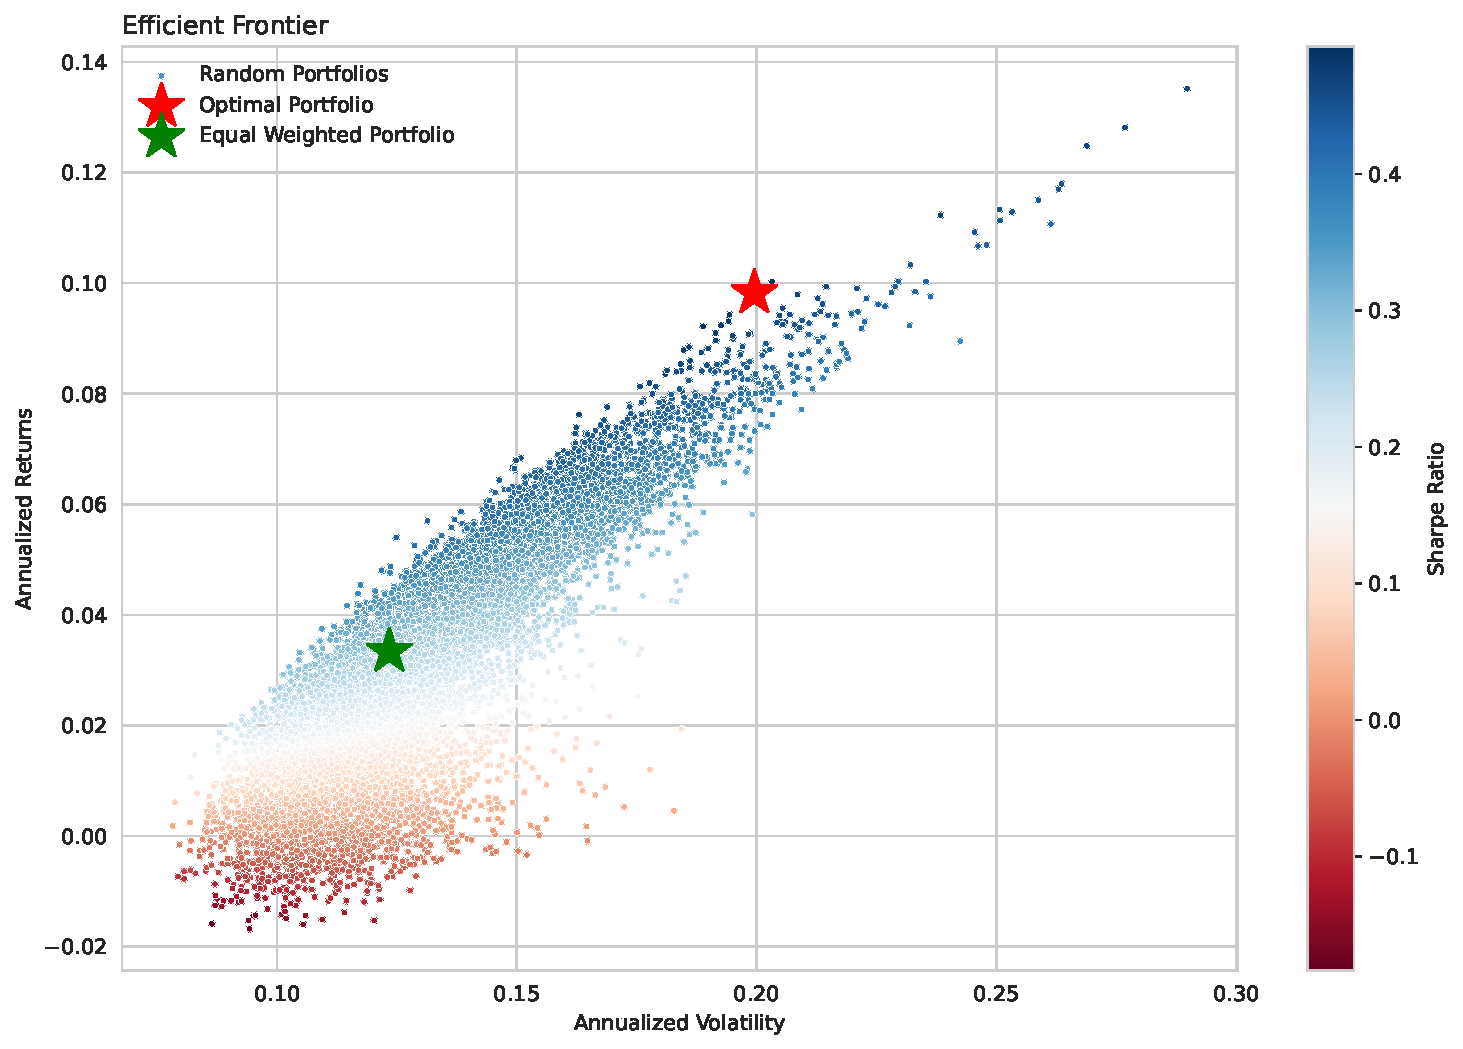
\includegraphics[width=1\textwidth]{paper/figure/Optimal_PF.pdf}
    \caption{Optimal Portfolio with Efficient Frontier.}
    \label{fig:mesh5}
\end{figure}

\newpage

\section{Conclusion and Outlook}

We have seen that a portfolio can be constructed considering the relationship between various asset classes and inflation. This portfolio, which is optimised according to Markowitz, significantly outperforms a simple, equally weighted portfolio. This analysis was done over a horizon of 9 years, including an economy with low inflation and a recent one with a high inflationary environment. \\

This optimisation can be done in many countries and specific sectors for further research. In this paper, we focused on the US with the US CPI data because of the sufficient data availability. In the future, with more data, this optimisation can also be carried out over a longer horizon with multiple inflationary environment cycles.

\end{document}
